\section{Analisi delle performance}
\label{cap:performance-analysis}

\subsection{Domanda \#1}

\begin{displayquote}
Eseguite i tre algoritmi che avete implementato (Held-Karp, 
euristica costruttiva e 2-approssimato) sui 13 grafi del dataset.
Mostrate i risultati che avete ottenuto in una tabella come quella
sottostante. Le righe della tabella corrispondono alle istanze del
problema. Le colonne mostrano, per ogni algoritmo, il peso della
soluzione trovata, il tempo di esecuzione e l'errore relativo 
calcolato come $(SoluzioneTrovata-SoluzioneOttima)/SoluzioneOttima$.
Potete aggiungere altra informazione alla tabella che ritenete 
interessanti.
\end{displayquote}

Per leggibilità la tabella richiesta è stata suddivisa nelle tabelle 
\ref{table:held-karp-runtime-accuracy},
\ref{table:mst2approx-runtime-accuracy},
\ref{table:farthest-insertion-runtime-accuracy}, 
una per algoritmo.

\begin{figure}[H]
    \centering

    \begin{tabular}{lrrrr}
    \toprule
    \multicolumn{2}{c}{ } & \multicolumn{3}{c}{Held Karp} \\
    \hline
    Instance & Exact & Solution &   Time (ms) &   Error (\%) \\
    \hline
    burma14.tsp   &     3323 &       3323 &          94 &        0    \\
    ulysses16.tsp &     6859 &       6859 &         393 &        0    \\
    ulysses22.tsp &     7013 &       7013 &       75295 &        0    \\
    eil51.tsp     &      426 &        986 &      126289 &      131.46 \\
    berlin52.tsp  &     7542 &      17441 &      126570 &      131.25 \\
    kroA100.tsp   &    21282 &     167464 &      128452 &      686.88 \\
    kroD100.tsp   &    21294 &     149007 &      128377 &      599.76 \\
    ch150.tsp     &     6528 &      48362 &      128392 &      640.84 \\
    gr202.tsp     &    40160 &      55127 &      128389 &       37.27 \\
    gr229.tsp     &   134602 &     176922 &      128344 &       31.44 \\
    pcb442.tsp    &    50778 &     512263 &      128303 &      908.83 \\
    d493.tsp      &    35002 &     321918 &      128277 &      819.71 \\
    dsj1000.tsp   & 18659688 &  546816520 &      128450 &     2830.47 \\
    \bottomrule
    \end{tabular}

    \caption{Held \& Karp runtime and accuracy}
    \label{table:held-karp-runtime-accuracy}
\end{figure}

\begin{figure}[H]
    \centering

    \begin{tabular}{lrrrr}
    \toprule
    \multicolumn{2}{c}{ } & \multicolumn{3}{c}{MST 2 Approximation} \\
    \hline
    Instance & Exact & Solution &   Time (ms) &   Error (\%) \\
    \hline
    burma14.tsp   &     3323 &       4258 &          33 &       28.14 \\
    ulysses16.tsp &     6859 &       7857 &          35 &       14.55 \\
    ulysses22.tsp &     7013 &       8377 &          36 &       19.45 \\
    eil51.tsp     &      426 &        563 &          36 &       32.16 \\
    berlin52.tsp  &     7542 &      10402 &          36 &       37.92 \\
    kroA100.tsp   &    21282 &      30032 &          36 &       41.11 \\
    kroD100.tsp   &    21294 &      28467 &          36 &       33.69 \\
    ch150.tsp     &     6528 &       9116 &          34 &       39.64 \\
    gr202.tsp     &    40160 &      52967 &          38 &       31.89 \\
    gr229.tsp     &   134602 &     178434 &          37 &       32.56 \\
    pcb442.tsp    &    50778 &      74254 &          42 &       46.23 \\
    d493.tsp      &    35002 &      45669 &          44 &       30.48 \\
    dsj1000.tsp   & 18659688 &   25703578 &          69 &       37.75 \\
    \bottomrule
    \end{tabular}

    \caption{MST 2 Approximation runtime and accuracy}
    \label{table:mst2approx-runtime-accuracy}
\end{figure}

\begin{figure}[H]
    \centering

    \begin{tabular}{lrrrr}
    \toprule
    \multicolumn{2}{c}{ } & \multicolumn{3}{c}{Farthest Insertion} \\
    \hline
    Instance & Exact & Solution &   Time (ms) &   Error (\%) \\
    \hline
    burma14.tsp   &     3323 &       3323 &          35 &        0    \\
    ulysses16.tsp &     6859 &       6859 &          35 &        0    \\
    ulysses22.tsp &     7013 &       7013 &          35 &        0    \\
    eil51.tsp     &      426 &        439 &          35 &        3.05 \\
    berlin52.tsp  &     7542 &       8118 &          36 &        7.64 \\
    kroA100.tsp   &    21282 &      23373 &          36 &        9.83 \\
    kroD100.tsp   &    21294 &      22577 &          36 &        6.03 \\
    ch150.tsp     &     6528 &       6864 &          41 &        5.15 \\
    gr202.tsp     &    40160 &      45211 &          46 &       12.58 \\
    gr229.tsp     &   134602 &     148324 &          52 &       10.19 \\
    pcb442.tsp    &    50778 &      56964 &         140 &       12.18 \\
    d493.tsp      &    35002 &      39506 &         176 &       12.87 \\
    dsj1000.tsp   & 18659688 &   20599827 &        1109 &       10.4  \\
    \bottomrule
    \end{tabular}

    \caption{Farthest Insertion runtime and accuracy}
    \label{table:farthest-insertion-runtime-accuracy}
\end{figure}

Una lettura più chiara dell'errore di approssimazione è invece
fornita dai grafici 
\ref{fig:heldkarp-mst2approx-farthestinsertion-accuracy-error-52-nodes}
 e \ref{fig:heldkarp-mst2approx-farthestinsertion-accuracy-error}. 
\'E possibile notare come nel
secondo grafico l'errore di approssimazione di HeldKarp diventi 
praticamente impredicibile, tendendo comunque a crescere con la
dimensione del grafo. Nel primo grafico invece è facile vedere
come l'algoritmo MST2Approximation sia l'unico ad avere errore
di approssimazione anche su taglie dell'input piccole,
come ci si aspettava.

\begin{figure}[H]
    \centering

    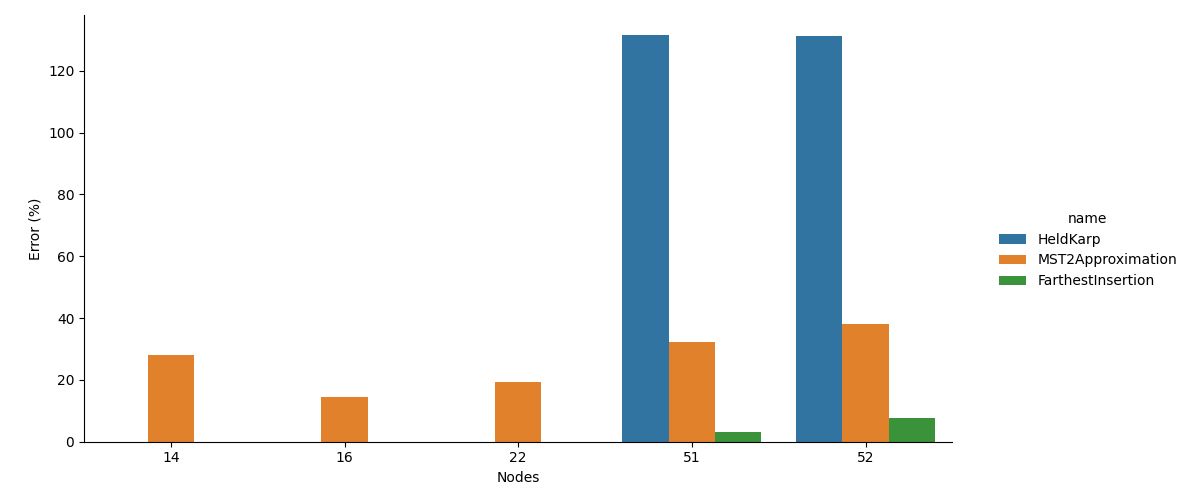
\includegraphics[width=0.9\textwidth]{./images/HeldKarp_vs_MST2Approximation_vs_FarthestInsertion__approximation_error__limited_to_52_nodes_.png}

    \caption{HeldKarp vs MST2Approximation vs FarthestInsertion accuracy error scaling by nodes (from 0 to 52 nodes)}
    \label{fig:heldkarp-mst2approx-farthestinsertion-accuracy-error-52-nodes}
\end{figure}

\begin{figure}[H]
    \centering

    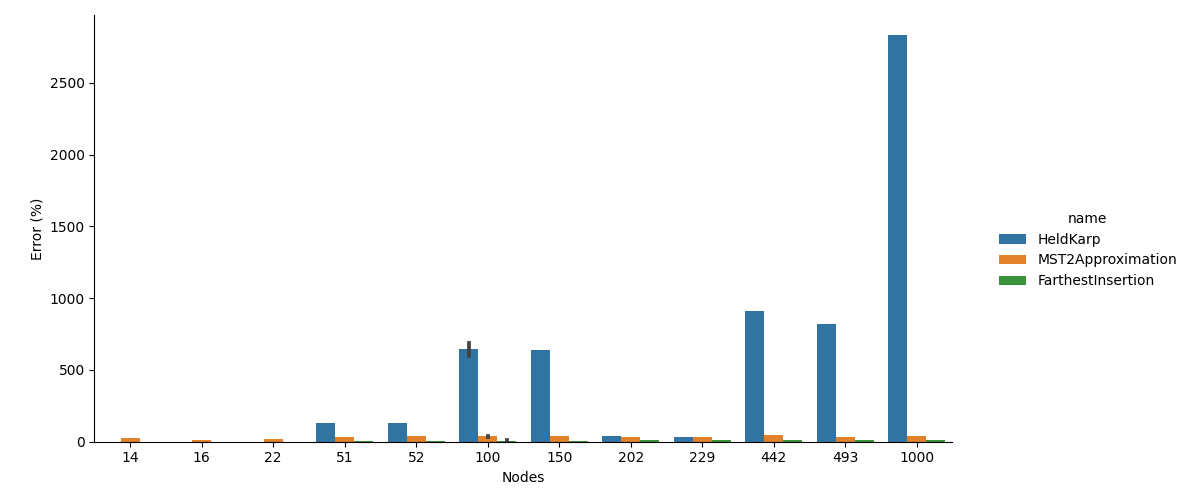
\includegraphics[width=0.9\textwidth]{./images/HeldKarp_vs_MST2Approximation_vs_FarthestInsertion__approximation_error_.png}

    \caption{HeldKarp vs MST2Approximation vs FarthestInsertion accuracy error scaling by nodes}
    \label{fig:heldkarp-mst2approx-farthestinsertion-accuracy-error}
\end{figure}

Il grafico che mostra i tempi di esecuzione non è stato inserito
in quanto ritenuto veramente poco informativo: HeldKarp va in 
timeout dopo i ventidue nodi (con il timeout fissato a due minuti),
mentre gli altri due algoritmi terminano in poco più di un secondo
su grafi di mille nodi. 

\subsection{Domanda \#2}

\begin{displayquote}
Commentate i risultati che avete ottenuto: come si comportano gli
algoritmi rispetti alle varie istanze? C'è un algoritmo che riesce
sempre a fare meglio degli altri rispetto all'errore di 
approssimazione? Quale dei tre algoritmi che avete implementato è
più efficiente?
\end{displayquote}


\noindent ---\\
